\level{2}{Processo di sviluppo}
		\level{3}{Studio di Fattibilità}
			Lo \insdoc{Studio di Fattibilità} deve essere rapido e accurato.\\
			Il documento di \insdoc{Studio di Fattibilità} viene redatto dagli analisti, sulla base di ciò che emerge dalle prime due riunioni. Qui i membri del gruppo si confrontano su tematiche riguardanti i capitolati quali:
			\begin{itemize}
				\item il dominio applicativo e tecnologico;
				\item il rapporto costi/benefici:
				\begin{itemize}
					\item confronto tra mercato attuale e futuro;
					\item costo di produzione e redditività dell'investimento;
				\end{itemize}
				\item i rischi ai quali essi sono soggetti.
			\end{itemize}

		\level{3}{Analisi dei Requisiti}
			Durante l'\insdoc{Analisi dei Requisiti} vengono catalogati e descritti tutti i requisiti che il \insglo{prodotto} dovrà possedere. Tali requisiti sono ottenuti da una delle seguenti fonti (presentate in ordine decrescente di importanza):
			\begin{enumerate}
				\item \insglo{capitolato} d’appalto;
				\item incontri con il proponente;
				\item incontri con il committente;
				\item valutazioni interne al gruppo di lavoro.
			\end{enumerate}
			Tali requisiti sono raccolti all'interno del documento \insdoc{Analisi dei Requisiti}. All'interno di tale documento è anche indicato un modo per verificare i requisiti in esso raccolti.
			\level{4}{Norme}
				\level{5}{Classificazione dei casi d'uso} \label{sec:classificazioneUC}
					I casi d'uso vengono identificati univocamente da una sigla nella forma UCYX.
					\begin{itemize}
						\item Y può assumere tre valori: N, A o D. N rappresenta tutti i casi d'uso inerenti a \insglo{Norris}, A rappresenta quelli inerenti l'applicazione \insglo{Android} e D rappresenta quelli che riguardano la \insglo{Dashboard}.
						\item X è un codice gerarchico numerico.
					\end{itemize}
					Sarà compito degli \insrole{analisti} identificare i casi d'uso e essi dovranno preoccuparsi di fornire un diagramma conforme allo standard \insglo{UML} per ogni caso d'uso non foglia. Qui di seguito sono riportate le informazioni da inserire nella parte testuale:
					\begin{itemize}
						\item titolo;
						\item attori (principali e secondari);
						\item precondizione;
						\item postcondizione;
						\item flusso principale degli eventi, dove si descrive il flusso dei casi d'uso figli; per ogni evento va specificato quanto segue:
						\begin{itemize}
							\item descrizione testuale;
							\item attori coinvolti;
							\item se l’evento è descritto nel dettaglio da un altro caso d’uso;
						\end{itemize}
						\item scenari alternativi; per ognuno di essi va specificato quanto segue:
						\begin{itemize}
							\item descrizione testuale;
							\item attori coinvolti;
							\item se lo scenario è descritto nel dettaglio da un altro caso d’uso.
						\end{itemize}
					\end{itemize}
				\level{5}{Classificazione dei requisiti}
					I requisiti dovranno essere classificati per tipo e importanza, utilizzando la seguente codifica: R[X][Y][Z].\\
					La codifica appena presentata deve essere interpretata nel modo seguente:
					\begin{enumerate}
						\item X indica l'importanza strategica del requisito e può assumere uno dei seguenti valori:
						\begin{itemize}
							\item R: requisiti obbligatori (required);
							\item D: requisiti desiderabili (desiderable);
							\item O: requisiti opzionali (optional).
						\end{itemize}
						\item Y indica la tipologia del requisito e può assumere i seguenti valori:
						\begin{itemize}
							\item F: indica che si tratta di un requisito funzionale (functional);
							\item P: indica che si tratta di un requisito prestazionale (performance);
							\item Q: indica che si tratta di un requisito di qualità (quality);
							\item C: indica che si tratta di un requisito di vincolo (constraint).
						\end{itemize}
						\item Z indica il codice gerarchico che identifica un requisito e dev'essere univoco.
					\end{enumerate}
	\level{4}{Strumenti}
		\level{5}{Software per la creazione di diagrammi UML}
			Per l'attività di Analisi dei Requisiti sono stati utilizzati i seguenti strumenti:
			\begin{itemize}
				\item per la creazione dei diagrammi \insglo{UML} è stato utilizzato il \insglo{software} \insglo{Astah};
				\item per la classificazione dei requisiti è stata utilizzata un'applicazione web creata dagli \insrole{Amministratori}.
			\end{itemize}
			Il \insglo{software} \insglo{Astah} è descritto nell'appendice \nameref{app:strumenti}, mentre l'applicazione per la classificazione dei requisiti è descritta nell'appendice \nameref{sec:tracker}.
			
	\level{3}{Progettazione}
		Scopo dell'attività di progettazione è produrre una soluzione soddisfacente per tutti i soggetti coinvolti nel progetto, una volta compreso esattamente quali sono i requisiti del problema. \\
		Approfondendo la progettazione del \insglo{prodotto} fino ad arrivare a moduli abbastanza semplici da essere capiti da una sola persona, si otterranno le istruzioni necessarie ai \insrole{Programmatori} per ottenere il \insglo{prodotto} finito.
			
		\level{4}{Progettazione architetturale}
			Prima di procedere alla definizione vera e propria dell'architettura dei vari prodotti software, devono essere eseguiti e successivamente documentati i seguenti task:
			\begin{enumerate}
				\item si individuano i prodotti che si intendono realizzare;
				\item si definiscono ruoli e responsabilità di ognuno dei prodotti individuati;
				\item si definiscono le interazioni che i prodotti hanno fra di loro;
				\item ci si assicura che ogni requisito sia soddisfatto da almeno uno dei prodotti individuati e descritti;
				\item ci si assicura che ogni prodotto realizzi almeno un requisito.
			\end{enumerate}
			A questo punto si può procedere con la progettazione dell'architettura dei prodotti software che si intendono realizzare. Si devono eseguire e successivamente documentare i seguenti task per ognuno dei prodotti individuati:
			\begin{enumerate}
				\item si suddivide il prodotto in componenti;
				\item si definisce il ruolo di ogni componente individuato;
				\item si definiscono le interazioni che i componenti hanno fra loro;
				\item si definiscono le eventuali interfacce che ogni componente mette a disposizione dell'ambiente esterno;
				\item ci si assicura che ogni requisito sia soddisfatto da almeno uno dei componenti individuati e descritti;
				\item ci si assicura che ogni componente realizzi almeno un requisito.
			\end{enumerate}
			Durante la suddivisione del prodotto in componenti è auspicabile che i \insrole{Progettisti} utilizzino in modo appropriato i design pattern. Qualora ciò dovesse avvenire, si documenta la cosa procedendo con una loro descrizione e contestualizzazione (per maggiori informazioni si consulti la sezione \nameref{sec:ProgDesingPattern}).\\
			Un utile supporto alla documentazione di tutti i task precedentemente descritti sono i diagrammi UML. Per maggiori informazioni si culsulti la sezione \nameref{sec:ProgUML}.\\
			Il modo in cui viene effettuato il tracciamento dei requisiti viene descritto in modo più approfondito nella sezione \nameref{sec:ProgTracCompReq}.
			\level{5}{Norme}
				\level{6}{Design Pattern} \label{sec:ProgDesingPattern}
					Al fine di consentire una migliore comprensibilità del documento, nonché delle scelte progettuali e della progettazione stessa, i \insrole{Progettisti} dovranno indicare i \insglo{pattern} architetturali impiegati, fornendo per ciascuno di essi:
					\begin{itemize}
						\item una descrizione testuale e grafica;
						\item la motivazione che ha portato alla sua scelta;
						\item una breve descrizione dell'applicazione del \insglo{pattern} al progetto.
					\end{itemize}
				\level{6}{Diagrammi UML} \label{sec:ProgUML}
					La documentazione riguardante i prodotti e i componenti individuati deve sempre fare uso di diagrammi \insglo{UML}. Essi sono necessari per esplicitare e formalizzare in modo migliore i vari aspetti che sono stati descritti testualmente.\\
					In particolare, durante la progettazione architetturale è necessario fare uso dei seguenti diagrammi:
					\begin{description}
						\item[diagrammi dei componenti] Essi hanno lo scopo di rappresentare la struttura interna di un prodotto software modellato in termini dei suoi componenti principali e delle relazioni fra di essi. Questo tipo di diagramma viene dunque utilizzato per evidenziare i componenti (e le relazioni che essi hanno fra di loro) individuati all'interno di ciascun prodotto software.
						\item[diagrammi delle attività] Essi hanno lo scopo di definire le attività da svolgere per realizzare una certa funzionalità. Vengono dunque usati per mostrare come determinate interazioni tra componenti (o fra prodotti) realizzino una funzionalità che si intende rendere disponibile.
					\end{description}
				\level{6}{Test di integrazione}
					Per ottenere maggior efficienza ed efficacia durante l'attività di test, è auspicabile che i \insrole{Progettisti} si preoccupino di definire delle classi di verifica per appurare che il funzionamento dei componenti sia quello previsto. Sarebbe infatti ideale poter fornire degli strumenti completamente automatici ai \insrole{Verificatori}.\\
					La progettazione delle classi per la verifica deve essere fatta da persone diverse da coloro che hanno progettato la classe da verificare, quando ciò fosse possibile.
			\level{5}{Strumenti}
				Per la progettazione architetturale sono stati utilizzati i seguenti strumenti:
				\begin{itemize}
					\item per la creazione dei diagrammi \insglo{UML} è stato utilizzato \insglo{Astah};
					\item per il tracciamento delle componenti è stata utilizzata l'applicazione web sviluppata dagli \insrole{Amministratori}.
				\end{itemize}
				Il \insglo{software} \insglo{Astah} è descritto in modo dettagliato nell'appendice \nameref{app:strumenti}, mentre l'applicazione web per il tracciamento viene descritta nell'appendice \nameref{sec:tracker}.
			\level{5}{Procedure}
				\level{6}{Tracciamento componenti-requisiti} \label{sec:ProgTracCompReq}
					È fondamentale che ogni requisito sia soddisfatto da uno e uno solo componente. Per controllare che ciò sia vero è necessario prima di tutto effettuare il tracciamento. Si seguano i passi descritti nella seguente procedura. Si noti che qui si da per scontato che i componenti e i requisiti siano già stati inseriti precedentemente sul Tracker del gruppo (per l'inserimento dei componenti fare riferimento alla procedura descritta nella sezione \nameref{sec:InsComponente}).
					\begin{enumerate}
						\item Accedere al Kaizen Team Tracker (\url{http://kaizenteam.it/tracker/}).
						\item Entrare all'interno della sezione “Requisiti”.
						\begin{figure}[H]
							\centering
							
\includegraphics[width=\textwidth]{Pics/HomePageMenuFrecciaReq}
						\end{figure}
						\item Scegliere uno dei requisiti ai quali si intende associare un componente e cliccare sul pulsante “Modifica”.
						\begin{figure}[H]
							\centering
							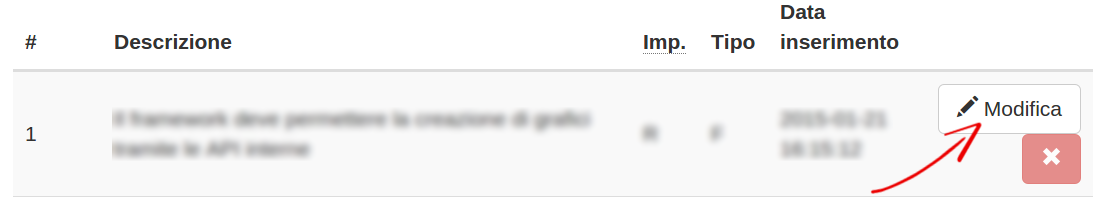
\includegraphics[width=\textwidth]{Pics/VistaRequisitoFrecciaModifica}
						\end{figure}
						\item Cercare la sezione “Componenti abbinati”. Scegliere dal menù a tendina il componente che realizza il requisito scelto al passo precedente. Cliccare sul pulsante “Aggiungi”. Un requisito  può essere associato a più componenti.
						\begin{figure}[H]
							\centering
							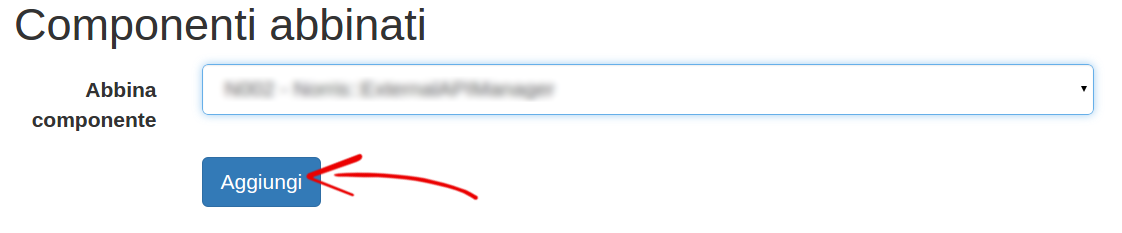
\includegraphics[width=\textwidth]{Pics/AbbianareComponenteRequisito}
						\end{figure}
						\item Eseguire il passo precedente per tutti i requisiti.
					\end{enumerate}
				\level{6}{Inserimento di un componente sul Tracker} \label{sec:InsComponente}
					Per poter effettuare correttamente i vari tracciamenti necessari si deve inserire all'interno del tracker del gruppo tutti i componenti che sono stati individuati dai \insrole{Progettisti} durante la progettazione architetturale. Per fare ciò si segua la seguente procedura.
					\begin{enumerate}
						\item Accedere al Kaizen Team Tracker (\url{http://kaizenteam.it/tracker/}).
						\item Entrare all'interno della sezione “Progettazione”.
						\begin{figure}[H]
							\centering
							
\includegraphics[width=\textwidth]{Pics/HomePageMenuFrecciaProg}
						\end{figure}
						\item Cliccare sul pulsante “Aggiungi componente”.
						\item Inserire il codice del componente che si desidera aggiungere e una sua descrizione (secondo le norme presenti nella sezione SEZIONE). Cliccare in seguito su “Salva”.
						\begin{figure}[H]
							\centering
							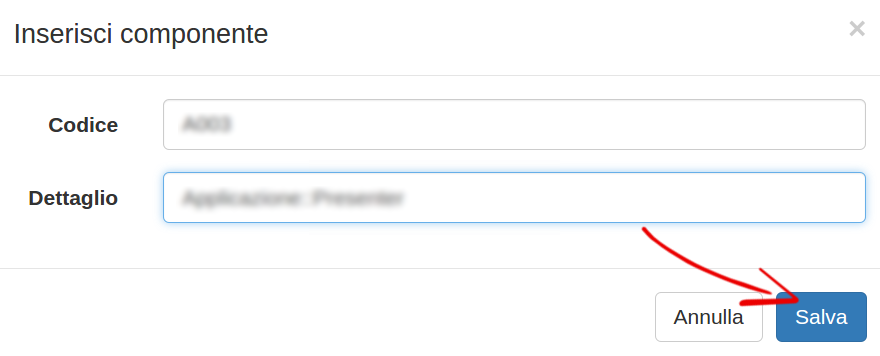
\includegraphics[width=\textwidth]{Pics/InserireComponente}
						\end{figure}
						\item Eseguire nuovamente i passi precedenti per inserire un nuovo componente all'interno del Tracker.
					\end{enumerate}

\level{4}{Progettazione di dettaglio}
La progettazione di dettaglio dei singoli componenti del \insglo{framework} \projectname{} viene descritta dai \insrole{Progettisti} nel documento \insdoc{Definizione di Prodotto v1.00}, avendo cura di rispettare i seguenti aspetti.
\level{5}{Norme}
\level{6}{Diagrammi UML}
Durante questa progettazione devono essere aggiornati con l'aggiunta di dettagli i seguenti diagrammi:
\begin{itemize}
\item diagrammi delle classi;
\item diagrammi di sequenza;
\item diagrammi delle attività.
\end{itemize}
Tali diagrammi dovranno seguire le indicazioni fornite nella sezione \nameref{sec:UML}.
\level{6}{Definizione di classe}
Ogni classe individuata dai \insrole{Progettisti} deve avere, oltre ad un proprio diagramma, una descrizione testuale contenente:
\begin{itemize}
\item il nome della classe completo dei \insglo{package} di cui fa parte;
\item la descrizione della classe con l'indicazione della sua funzione nel contesto del \insglo{package} a cui appartiene;
\item le sue relazioni con altre classi;
\item l'elenco dei metodi accompagnati da una breve ma significativa descrizione;
\item l'elenco degli attributi.
\end{itemize}
\level{6}{Test di unità}
I \insrole{Progettisti} devono definire i test di unità necessari per verificare che il funzionamento delle classi sia quello previsto.
\level{5}{Strumenti}
Per la progettazione di dettaglio è stato utilizzato il \insglo{software} \insglo{Astah}, descritto nell'appendice \nameref{app:strumenti}, per la creazione dei diagrammi \insglo{UML}.

\level{3}{Codifica} \label{sec:codifica}
L'attività di codifica ha lo scopo di produrre il codice necessario alla realizzazione del \insglo{prodotto} richiesto. Il codice generato dovrà rispettare il più fedelmente possibile ciò che è stato definito nel documento \insdoc{Definizione di Prodotto v1.00}.
	\level{4}{Norme}
	Tutti i file di codice devono seguire quanto riportato nella sezione \nameref{sec:CodificaFile} e le seguenti regole generali:
	\begin{itemize}
		\item l'indentazione del codice deve essere di quattro spazi;
		\item le righe non devono essere più lunghe di 80 caratteri;
		\item i commenti devono essere scritti in lingua inglese e devono essere significativi;
		\item ogni file, sia \insglo{JavaScript} che \insglo{Java}, deve iniziare con un'intestazione che rifletta la seguente struttura:
		\begin{lstlisting}
			/*
			* Name: [nome del file]
			* (*\ignoreglo{Package}*): [(*\ignoreglo{package}*) al quale appartiene il file]
			* Location: [path della directory di appartenenza]
			* Date: [data di creazione del file]
			* Version: [versione del file]
			* 
			* History:
			* 
			* =================================================================
			* Version  Date        Programmer    Changes
			* =================================================================
			* v0.01    AAAA-MM-GG  Nome Cognome  {descrizione modifica}
			* =================================================================
			*
			*/
		\end{lstlisting}
		dove:
		\begin{description}
			\item[Name] indica il nome del file comprensivo di estensione;
			\item[\ignoreglo{Package}] indica il \insglo{package} al quale appartiene il file, comprensivo di gerarchia;
			\item[Location] indica il path della directory in cui è presente il file;
			\item[Date] indica la data di creazione del file: si veda la sezione \nameref{sec:formatoDate} per il formato da utilizzare;
			\item[Version] indica l'attuale versione del codice, il cui formato da seguire è descritto nella sezione \nameref{sec:versioni};
			\item[History] visualizza lo storico delle modifiche del file in questione, comprensive di versione, data, descrizione e nome del programmatore che ha modificato il codice.
		\end{description}
	\end{itemize}
		\level{5}{JavaScript}
		Ciascun file \insglo{JavaScript}, oltre a seguire le norme precedentemente descritte, deve rispettare, anche, le linee guida \textit{Google \insglo{JavaScript} Style Guide} reperibili all'indirizzo \insuri{https://google-styleguide.googlecode.com/svn/trunk/javascriptguide.xml}. 
		\level{5}{Java}
		Ciascun file \insglo{Java}, oltre a rispettare le norme sopra citate, deve seguire le linee guida \textit{Google \insglo{Java} Style Guide} reperibili all'indirizzo \insuri{https://google-styleguide.googlecode.com/svn/trunk/javaguide.html}. 
	\level{4}{Strumenti}
	Per la scrittura di codice \insglo{JavaScript} non è richiesto l'utilizzo di un particolare \insglo{IDE}; la scelta dell'editor di testo è a discrezione dello sviluppatore.
		\level{5}{Android Studio}
		Per lo sviluppo dell'applicazione \insglo{Android} si utilizza l'\insglo{IDE} \insglo{Android} Studio, descritto nell'appendice \nameref{app:strumenti} del presente documento.
